\documentclass[mathpazo]{cicp}

%\journal{Applied Mathematics and Computation}
\usepackage{graphicx}
\usepackage{amssymb}
\usepackage{amsmath}
\usepackage{amsthm}
\usepackage{amssymb}
\usepackage{amsfonts}
\usepackage{amsrefs}
%\usepackage{subfig}

\begin{document}

%\title{\emph{hp}-Finite Element Model of Poisson and Nernst-Planck\\ System of Equations}
\title{Modeling Ionic Polymer-Metal Composites\\ with Space-Time Adaptive Multimesh \emph{hp}-FEM}


\author[Deivid Pugal et.~al.]{Deivid Pugal\affil{1}\comma\affil{4},
Pavel Solin\affil{2}\comma\affil{3}\comma\corrauth,
Kwang J. Kim\affil{1}, and Alvo Aabloo\affil{4}}

\address{\affilnum{1}\ Mechanical Engineering Department, University of Nevada, Reno, NV, U.S.A.\\
\affilnum{2}\ Department of Mathematics and Statistics, University of Nevada, Reno, NV, U.S.A.\\
\affilnum{3}\ Institute of Thermomechanics, Prague, Czech Republic\\
\affilnum{4}\ Institute of Technology, Tartu University, Estonia}

\emails{{\tt david.pugal@gmail.com} (D.~Pugal), {\tt solin@unr.edu} (P.~Solin),
	{\tt kwangkim@unr.edu} (K.~Kim), {\tt alvo@ut.ee} (A.~Aabloo)}

%\author[unrme,tartu]{D.~Pugal}
%\ead{david.pugal@gmail.com}
%
%\author[unrmath,czech]{P.~Solin\corref{cor2}}
%\ead{solin@unr.edu}
%
%\author[unrme]{K.~J.~Kim\corref{cor1}}
%\ead{kwangkim@unr.edu}
%
%\author[tartu]{A.~Aabloo}
%\ead{alvo@ut.ee}
%
%\address[unrme]{Mechanical Engineering Department, University of Nevada, Reno, NV, U.S.A.}
%\address[unrmath]{Department of Mathematics and Statistics,
%University of Nevada, Reno, NV, U.S.A.}
%\address[czech]{Institute of Thermomechanics, Prague, Czech Republic}
%\address[tartu]{Institute of Technology, Tartu University, Estonia}
%
%\cortext[cor1]{Corresponding author}
%\cortext[cor2]{Principal corresponding author}

\begin{abstract}
We are concerned with a model of ionic polymer-metal composite (IPMC) materials
that consists of a coupled system of the Poisson and Nernst-Planck equations, 
discretized by means of the finite element method (FEM). We show that due to the 
transient character of the problem it is efficient to use adaptive algorithms 
that are capable of changing the mesh dynamically in time. We also show 
that due to large qualitative and quantitative differences between the 
two solution components, it is efficient to approximate them on different 
meshes using a novel adaptive multimesh \emph{hp}-FEM. The study is 
accompanied with numerous computations and comparisons of the adaptive 
multimesh \emph{hp}-FEM with several other adaptive FEM algorithms. 
\end{abstract}

%\begin{keyword}
%\keywords{Ionic polymer-metal composites, IPMC, Nernst-Planck equation, Poisson equation,
%finite element method, space-time adaptivity, multimesh \emph{hp}-FEM }
%\end{keyword}

%see http://www.ams.org/mathscinet/msc/msc2010.html?t=35Qxx&btn=Current

\ams{35Q84, 35Q05, 35J47}
\keywords{Ionic polymer-metal composites, IPMC, Nernst-Planck equation, Poisson equation,
finite element method, FEM, adaptive multimesh \emph{hp}-FEM }
\maketitle


%\end{frontmatter}

\section{Introduction}

Ionic Polymer-Metal Composites (IPMC) have been studied during the past two 
decades for their potential to serve as noiseless mechanoelectrical and electromechanical transducers.
The advantages of IPMC over other electroactive polymer actuators
are low voltage bending, high strains ($>1\%$), and an ability to work
in wet environments. A typical IPMC consists of a thin sheet of polymer
(often Nafion or Teflon) which is sandwiched between noble
metal electrodes such as platinum or gold. When fabricated, the polymer 
membrane is saturated with certain solvent and ions such as water and $H^+$.
When a voltage is applied to the electrodes, the counter ions start
migrating due to the imposed electric field. By dragging along the solvent,
the osmotic pressure difference near the electrodes
results in bending of the material (see Fig.~\ref{fig:conceptual}).
\begin{figure}[!ht]
  \begin{centering}
    \subfloat[~]{\begin{centering}
      \includegraphics[scale=0.6]{IPMC}
      \par\end{centering}}~
    \subfloat[~]{\begin{centering}
      \includegraphics[scale=0.6]{IPMC_bent}
      \par\end{centering}}
  \par\end{centering}
  \caption{\label{fig:conceptual}Conceptual model of the actuation
 	of IPMC. Initial counter ion distribution (a) and
	the distribution and resulting bending after applying a voltage (b).}
\vspace{-1cm}
\end{figure}
\newpage
%The derived and implemented model helps to predict the actuation of the
%material. Furthermore, it is expected that the \emph{hp}-FEM implementation
%results in a smaller problem size, thus likely allowing faster calculation
%in both 2D and 3D domains.

In this study we will model IPMC materials via a multiphysics coupled problem 
consisting of the Poisson and Nernst-Planck equations (abbreviated by PNP in
the following). These equations are used to model charge transport in materials 
that includes ionic migration, diffusion, and convection. The charge transport 
process is a key mechanism for electromechanical transduction 
\cite{basu1997membrane,shahinpoor2001smartmat,
nasser2002applied,newbury2003intelligent, wallmersperger2007appliedphysics,
pugal2008appliedphysics,pugal2010polymer}.

The PNP system is highly nonlinear and for a typical domain with two
electrodes, largest differences in charge concentration occur in a very narrow
region near the boundary. The computing power required for a full scale problem 
is significant. This is why we are interested in exploring adaptive algorithms
-- we hope to obtain meshes that are optimal in terms of calculation time and 
calculation error.

The Nernst-Planck equation for a mobile species ---
in our case for counter ions --- has the form
\begin{equation}
  \frac{\partial C}{\partial t}+\nabla\cdot(-D\nabla C-z\mu FC\nabla\phi)=0.
  \label{eq:nernst-planck}
\end{equation}
Here $C$ stands for the counter ion concentration, $D$ is diffusion, $\mu$ mobility,
$F$ Faraday constant, $\phi$ voltage, and $z$ the charge number. We have neglected 
the velocity of the species as in our case it can be assumed zero. 
The Poisson equation has the form
\begin{equation}
  -\nabla^2\phi=\frac{F\rho}{\varepsilon}
  \label{eq:poisson}
\end{equation}
where $\varepsilon$ is the absolute dielectric permittivity. The
charge density $\rho$ is defined via
\begin{equation}
  \rho=C-C_{0}
  \label{eq:rho}
\end{equation}
where $C_{0}$ is a constant anion concentration.

The outline of the paper is as follows: Section \ref{sec:moti} shows that 
the solution components $C$ and $\phi$ have very different behavior, which
is the reason why it is difficult to find a common mesh that would be optimal 
for each of them. This explains why we are interested in applying the novel
multimesh $hp$-FEM method~\cite{solin2010monolithic,solin2010adaptive,dubcova2010space}.
The PNP model is presented in Section \ref{sec:model} where also its weak 
formulation for the Newton's method is derived. Section \ref{sec:hermes}
describes briefly the open source adaptive $hp$-FEM library Hermes
that is used to solve the problem numerically. 
Numerical results and comparisons are presented in Section \ref{sec:results},
and conclusion and outlook are drawn in Section \ref{sec:conc}.



\section{Motivation} \label{sec:moti}

In this section we use a simplified one-dimensional model to illustrate the 
principal difficulties encountered in the numerical solution of the 
PNP system.
Table~\ref{Table:used-constants} shows constants that we will use in 
computations in this section as well as in the rest of the paper: 

\begin{table}[!ht]
\caption{Constants used in the Poisson-Nernst-Planck system of equations.}
\centering
\label{Table:used-constants}
{
\begin{tabular}{llll}
  \hline \hline
  Constant&Value&Unit&Description\\
  \hline
  $D$&$10\times10^{-11}$&$\frac{m^2}{s}$&Diffusion constant\\
  $z$&1&-&Charge number\\
  $F$&96,485&$\frac{C}{mol}$&Faraday number\\
  $R$&8.31&$\frac{J}{mol\cdot K}$&The gas constant\\
  $\mu\ \left( = \frac{D}{RT}\right)$&$4.11\times 10^{-14}$&$\frac{s}{mol\cdot K}$&Mobility\\
  $C_{0}$&1,200&$\frac{mol}{m^3}$&Anion concentration\\
  $\varepsilon$&0.025&$\frac{F}{m}$&Electric permittivity\\
  \hline
  \hline
\end{tabular}
}
\end{table}


Fig.~\ref{fig:comsol-conc-volt} shows a typical solution for $C$ and $\phi$
at $t=0.1\ s$ and $t=3.0\ s$. 
The solution has 
two notable characteristics: For the most part of the domain $\Omega$,
the gradient $\nabla C = 0$. Close to $\partial \Omega_2$, $\nabla C$ is
nonzero and moving in time, and $\nabla C$ is very large at $\partial \Omega_1$.
At the same time, $\phi$ is a "nice" smooth function for the most part of 
$\Omega$ but it has a large gradient at $\partial \Omega_2$.
This makes the choice of an optimal mesh extremely difficult. Even if the 
solution was stationary, an optimal mesh for $C$ could never be 
optimal for $\phi$ and vice versa.


\begin{figure}[!ht]
  \begin{centering}
      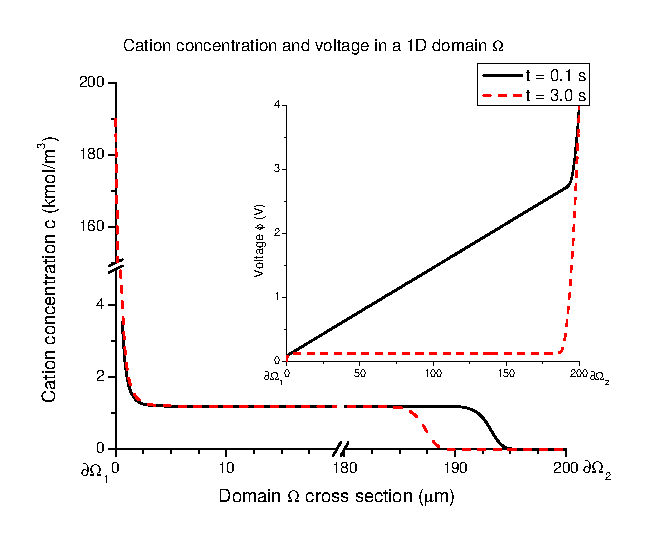
\includegraphics{comsol_conc_volt}
      %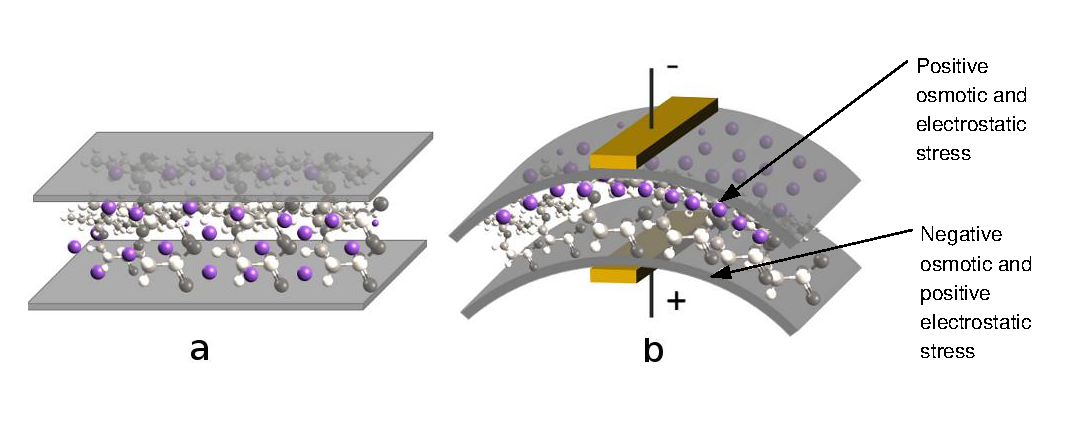
\includegraphics{IPMC_bending}
  \caption{Sample concentration $C$ and voltage $\phi$
           in a 1D domain $\Omega\subset\mathbb{R}$.
           Dirichlet boundary conditions ($V_{\partial \Omega_1}=0\ V$
           and $V_{\partial \Omega_2}=4\ V$) were
	   applied to the Poisson equation \eqref{eq:poisson} and Neumann conditions
	   to the Nernst-Planck equation \eqref{eq:nernst-planck}.}
\label{fig:comsol-conc-volt}
  \end{centering}
\end{figure}



Furthermore, the shape of the solution in Fig.~\ref{fig:comsol-conc-volt}
suggests that the polynomial degree of finite elements in the middle
of the domain $\Omega$ and near the boundaries $\partial \Omega_1,\ \partial \Omega_2$
should be different --- large high-degree elements should be used in the middle of the 
domain while small low-degree ones should be used in the boundary layers.  
The qualitative differences in the solution components $C$ and $\phi$ 
also suggest that using different meshes would be beneficial. 

% THIS DOES NOT BELONG HERE
%All the aforementioned concerns can be solved by using
%a time dependent adaptive multimesh \emph{hp}-FEM solver.
%Automatic time dependent adaptivity in conjuction with \emph{hp}-FEM 
%helps to limit the error of the calculations by automatically choosing
%a suitable mesh and polynomial degrees of the elements at each time step.
%In this work Hermes~\cite{Hermes-project} was used to implement
%the PNP system and study
%the problem size, error convergence and solution time 
%with different refinement modes.




\newpage
\section{Model}\label{sec:model}

We consider a rectangular 2D domain $\Omega\subset\mathbb{R}^2$ with boundaries 
$\partial\Omega_{1\ldots 4}\subset\partial\Omega$, shown in Fig.~\ref{fig:domain}.

\begin{figure}[!ht]
  \begin{centering}
  \includegraphics[width=0.2\columnwidth]{domain}
  \caption{\label{fig:domain} Calculation domain $\Omega\subset\mathbb{R}^2$
  	with boundaries $\partial\Omega_{1\ldots 4}\subset\partial\Omega$.}
  \end{centering}
\end{figure}

As there is no flow through the domain's boundary, Eq.~\eqref{eq:nernst-planck}
is equipped with a Neumann boundary condition 
\begin{equation}
  -D \frac{\partial C}{\partial n} - \mu F C \frac{\partial \phi} {\partial n} = 0.
  \label{eq:nernst-planck-boundary}
\end{equation}
Furthermore, we prescribe a positive constant voltage $V_{pos}$ 
on $\Omega_1$ and zero voltage on $\Omega_3$:
\begin{eqnarray}
  \phi_{\partial\Omega_1}&=&V_{pos},\\
  \phi_{\partial\Omega_3}&=&0.
  \label{eq:dirichlet}
\end{eqnarray}
On the rest of the boundary, $\phi$ has zero normal derivatives, and thus we prescribe 
a Neumann boundary condition
\begin{equation}
  \frac{\partial \phi_{\Omega_2}}{\partial n}=\frac{\partial \phi_{\Omega_4}}{\partial n}=0.
\end{equation}


\subsection{Weak form of the PNP system}

To make our results easily reproducible, in the following we present the derivation 
of weak forms of Eqs.~\eqref{eq:nernst-planck} and 
\eqref{eq:poisson}, as well as formulas for the Jacobian matrix and residual 
vector that are used in actual computations.
To simplify notation, we use dimensionless formulation of Eqs.~\eqref{eq:nernst-planck}
and~\eqref{eq:poisson}. The following new notations for the independent variables
$x$, $y$, $t$ and for the dependent variables $C$ and $\phi$ are used~\cite{bazant2004diffuse}:
\begin{equation}
  X=\frac xl,\ \ \
  Y=\frac yl,\ \ \
  \tau=\frac{tD}{\lambda_D l},\ \ \
  \varphi=\frac{\phi F}{RT},\ \ \
  c=\frac C C_0.\label{eq:dimensionless}
\end{equation}
Here $\lambda_D$ is the Debye screening length and it is expressed as follows~\cite{bazant2004diffuse}:
\begin{equation}
  \lambda_D=\sqrt{\frac{\varepsilon R T}{2 F^2 C_0}}.\label{eq:debye}
\end{equation}
After inserting variables~\eqref{eq:dimensionless} into Eq.~\eqref{eq:nernst-planck} the Nernst-Planck
equation and Poisson equation become:
\begin{eqnarray}
  \frac{DC_0}{\lambda_D l}\frac{\partial c}{\partial \tau} + \frac 1l  \nabla_d\cdot
    \left(-\frac{DC_0}{l}\nabla_dc-c\frac{DC_0}{l}\nabla_d\varphi\right) &=& 0\label{eq:dim1}\\
  - \frac{\varepsilon R T}{l^2F^2C_0}\nabla_d^2\varphi&=&c-1\label{eq:dim2},
\end{eqnarray}
where
\begin{equation}
  \nabla_d=\left(\frac{\partial}{\partial X},\ \frac{\partial}{\partial Y}\right).
\end{equation}
After simplifying Eqs.~\eqref{eq:dim1} and~\eqref{eq:dim2} and denoting
\begin{equation}
  \epsilon=\frac{\lambda_D}{l},
\end{equation}
the dimensionless form of the PNP system of equations is
\begin{eqnarray}
  \frac{\partial c}{\partial \tau}
    -\epsilon\nabla_d^2 c - \epsilon \nabla_d \cdot \left( c\nabla_d \varphi\right)  &=&0,\label{eq:dimensionless-nernst-planck}\\
  -\nabla_d^2\varphi&=&\frac{c-1}{2\epsilon^2}\label{eq:dimensionless-poisson}.
\end{eqnarray}
Boundary condition Eq.~\eqref{eq:nernst-planck-boundary} has the form
\begin{equation}
  -\frac{\partial c}{\partial n}-c\frac{\partial\varphi}{\partial n}=0.
  \label{eq:dimensionless-nernst-planck-boundary}
\end{equation}
As the second derivatives of both $c$ and $\varphi$ are present in the 
equations, the appropriate function space for them is the Sobolev space 
$V=H^1\left(\Omega\right)$ where 
$$H^1\left(\Omega\right)=\left\{v\in L^2\left(\Omega\right);\ \nabla_d v \in \left[L^2\left(\Omega\right)\right]^2\right\}.
$$
In order to derive the weak form of the Nernst-Planck equation Eq.~\eqref{eq:dimensionless-nernst-planck},
we first multiply it with a test function $v^c \in V$ and integrate over the domain~$\Omega$,
\begin{equation}
  \int_{\Omega}\frac{\partial c}{\partial \tau}v^c d\mathbf{x}-
  \int_{\Omega}\epsilon\nabla_d^2cv^c d\mathbf{x}-\int_{\Omega}\epsilon\nabla_d c\cdot\nabla_d\varphi v^c d\mathbf{x}-
  \int_{\Omega}\epsilon c\nabla_d^2\varphi v^c d\mathbf{x}=0.
  \label{eq:nernst-planck-weak1}
\end{equation}
Applying the Green's first identity to the terms that contain second derivatives,
we obtain
$$
 \int_{\Omega}\frac{\partial c}{\partial \tau}v^c d\mathbf{x}+
  \epsilon\int_{\Omega}\nabla_d c\cdot\nabla_d v^c d\mathbf{x}-
  \epsilon\int_{\Omega}\nabla_d c\cdot\nabla_d\varphi v^c d\mathbf{x}
$$
\begin{equation}
  + \epsilon\int_{\Omega}\nabla_d\left(cv^c\right)\cdot \nabla_d \varphi d\mathbf{x}
  -\epsilon\int_{\partial\Omega}\frac{\partial c}{\partial n}v^c d\mathbf{S}-
  \int_{\partial\Omega}\epsilon\frac{\partial\varphi}{\partial n}cv^c d\mathbf{S}=0.
  \label{eq:nernst-planck-weak2}
\end{equation}
Expanding the nonlinear term and using the boundary condition 
\eqref{eq:dimensionless-nernst-planck-boundary}, we have
$$
  \int_{\Omega}\frac{\partial c}{\partial \tau}v^c d\mathbf{x}+
  \epsilon\int_{\Omega}\nabla_d c\cdot\nabla_d v^c d\mathbf{x}-
  \epsilon\int_{\Omega}\nabla_d c\cdot\nabla_d\varphi v^c d\mathbf{x}
$$
\begin{equation}
  + \epsilon\int_{\Omega}\nabla_d \varphi \cdot \nabla_d c v^c d\mathbf{x}+
  \epsilon \int_{\Omega} c \left(\nabla_d\varphi\cdot\nabla_d v^c\right) d\mathbf{x}=0.
  \label{eq:nernst-planck-weak3}
\end{equation}
After the third and fourth terms cancel out, we obtain the final weak form of 
the Nernst-Planck equation
\begin{equation}
  \int_{\Omega}\frac{\partial c}{\partial \tau}v^c d\mathbf{x}+
  \epsilon\int_{\Omega}\nabla_d c\cdot\nabla_d v^c d\mathbf{x}+
  \epsilon \int_{\Omega} c \left(\nabla_d\varphi\cdot\nabla_d v^c\right) d\mathbf{x}=0.
  \label{eq:nernst-planck-weak-final}
\end{equation}
Analogously we derive also the weak form of the Poisson equation (\ref{eq:dimensionless-poisson}),
\begin{equation}
  -\int_{\Omega}\nabla_d^2\varphi v^\varphi d\mathbf{x}-
  \frac{1}{2\epsilon^2}\left[\int_{\Omega}cv^\varphi d\mathbf{x}-
  \int_{\Omega}v^\varphi d\mathbf{x}\right]=0.
  \label{eq:poisson-weak1}
\end{equation}
Performing integration by parts and taking into account the boundary 
conditions for $\varphi$, we obtain
\begin{equation}
  \int_{\Omega}\nabla_d\varphi\cdot\nabla_d v^\varphi d\mathbf{x}-
  \frac{1}{2\epsilon^2}\left[\int_{\Omega}cv^\varphi d\mathbf{x}-
  \int_{\Omega}v^\varphi d\mathbf{x}\right]=0.
  \label{eq:poisson-weak-final}
\end{equation}


\subsection{Jacobian matrix and residual vector for the Newton's method}
To employ the Newton's method for the nonlinear system \eqref{eq:nernst-planck-weak-final},
\eqref{eq:poisson-weak-final}, formulas for the Jacobian matrix and residual vector need to
be derived. Time discretization will be performed using the second-order Crank-Nicolson 
method. The unknown solution components 
$c^{n+1}$ and $\varphi^{n+1}$ at the end of the time step $\delta\tau$ are expressed 
as linear combinations of finite element basis functions $v_k^{c}$ 
and $v_k^{\varphi}$ with unknown coefficients,
\begin{eqnarray}
  c^{n+1} = c(Y^{n+1}) &=& \sum_{k=1}^{N^c} y_k^{c} v_k^{c}, \label{eq:cnotation}\\
  \varphi^{n+1} = \varphi(Y^{n+1}) &=& \sum_{k=1}^{N^{\varphi}} y_k^{\varphi} v_k^{\varphi}\label{eq:phinotation}.
\end{eqnarray}
Here $Y^{n+1}$ is a coefficient vector of length $N^c + N^{\varphi}$ comprising the unknown 
solution coefficients $y_k^{C}$ and $y_k^{\varphi}$ (in this order). We will also be 
using $c^n = c(Y^n)$ and $\varphi^n = \varphi(Y^n)$ for the previous time step solutions.

With the notation~\eqref{eq:cnotation}, \eqref{eq:phinotation}, the time discretized 
Eq.~\eqref{eq:nernst-planck-weak-final} leads to the formula for the 
first part $F^c$ of the residual vector $F$,
\begin{eqnarray}
  F_i^c\left(Y\right) & = & \int_{\Omega} \frac{c(Y)}{\delta\tau}v_i^c d\mathbf{x} - 
  \int_{\Omega} \frac{c^{n}}{\delta\tau}v_i^c d\mathbf{x}\nonumber\\
  &&+\frac 12 \epsilon \left[\int_{\Omega} \nabla_d c(Y) \cdot \nabla_d v_i^c d\mathbf{x}+ 
  	\int_{\Omega} \nabla_d c^{n} \cdot \nabla_d v_i^c d\mathbf{x}\right.\nonumber\\
  &&+ \left.\int_{\Omega}c(Y) \left(\nabla_d \varphi(Y) \cdot \nabla_d v_i^c\right) d\mathbf{x}+
  \int_{\Omega}c^{n} \left(\nabla_d \varphi^{n} \cdot \nabla_d v_i^c\right) d\mathbf{x}\right]\label{eq:Fc}
\end{eqnarray}
where $i = 1, 2, \ldots, N^c$.
Analogously, Eq.~\eqref{eq:poisson-weak-final} defines the second part $F^{\varphi}$ 
of the residual vector $F$,
\begin{equation}
  F_i^{\varphi}\left(Y\right) = \int_{\Omega} \nabla_d \varphi(Y) \cdot \nabla_d v_i^{\varphi} d\mathbf{x} 
  -\frac{1}{2\epsilon^2}\left[ \int_{\Omega} c(Y)v_i^{\varphi} d\mathbf{x} -
   \int_{\Omega} v_i^{\varphi} d\mathbf{x}\right]
  \label{eq:Fphi}
\end{equation}
where $i = N^c + 1, N^c + 2, \ldots, N^c + N^{\varphi}$. The nonlinear discrete problem 
that needs to be solved at the end of each time step thus has the form 
$F(Y) = 0$.

%\newpage

\noindent
The Jacobian matrix $J(Y) = DF/DY$ has a $2\times 2$ block structure,
\begin{equation}
J(Y) = \left(
\begin{array}{cc}
  \displaystyle \frac{\partial F_i^c}{\partial y_j^c} & \displaystyle \frac{\partial F_i^c}{\partial y_j^{\varphi}} \\ 
  \displaystyle \frac{\partial F_i^{\varphi}}{\partial y_j^c} & \displaystyle \frac{\partial F_i^{\varphi}}{\partial y_j^{\varphi}}
\end{array}
\right),
\end{equation}
and its entries are obtained by calculating the partial derivatives of $F$ with
respect to the components of the coefficient vector $Y$. For this it is useful to 
realize that 
$$
\frac{\partial c(Y)}{\partial y_j^c} = v_j^c, \ \ \ 
\frac{\partial \nabla_d c(Y)}{\partial y_j^c} = \nabla_d v_j^c,\ \ \ \mbox{etc.}.
$$
We obtain
\begin{eqnarray}
  \frac{\partial F_i^c}{\partial y_j^c}(Y) &=& 
  \int_{\Omega} \frac{1}{\delta\tau} v_j^c v_i^c d\mathbf{x} + 
  \frac 12 \epsilon\left[\int_{\Omega} \nabla_d v_j^c \cdot \nabla_d v_i^c d\mathbf{x}
  + \int_{\Omega} v_j^c \left(\nabla_d \varphi(Y) \cdot \nabla_d v_i^c\right) d\mathbf{x}\right],\label{eq:dFcdyc}\\
  \frac{\partial F_i^c}{\partial y_j^{\varphi}}(Y) &=&
  \frac 12 \epsilon \int_{\Omega} c(Y) \left(\nabla_d v_j^{\varphi} \cdot \nabla_d v_i^c\right) d\mathbf{x},\\
  \frac{\partial F_i^{\varphi}}{\partial y_j^c}(Y) &=&
  - \frac{1}{2\epsilon^2}\int_{\Omega} v_j^c v_i^{\varphi} d\mathbf{x},\\
  \frac{\partial F_i^{\varphi}}{\partial y_j^{\varphi}}(Y) &=&
  \int_{\Omega} \nabla_d v_j^{\varphi} \cdot \nabla_d v_i^{\varphi} d\mathbf{x}\label{eq:dFphidyphi}.
\end{eqnarray}

\subsection{Newton's iteration}
At the beginning of the $(n+1)$st time step we 
set $Y^{n+1}_0 = Y^n$, where $Y^n$ is the coefficient vector  
that was calculated in the $n$th time step (or coming from the 
initial condition if $n = 0$). We set $k = 0$ and run the 
Newton's iteration 
\begin{eqnarray*}
J(Y^{n+1}_k) \delta\tau Y^{n+1}_{k+1} &=& -F(Y^{n+1}_k), \\ 
Y^{n+1}_{k+1} &=& Y^{n+1}_k + \delta\tau Y^{n+1}_{k+1}, \\
k &:=& k+1
\end{eqnarray*}
over $k$ until it converges. Then we set $Y^{n+1} := Y^{n+1}_{k}$. 
We use a combined stopping criterion 
that makes sure that both the norm of the residual vector $\Vert F(Y^{n+1})\Vert$ 
as well as the norm of the increment $\Vert \delta Y^{n+1}\Vert$ are sufficiently 
small.

\section{Adaptive $hp$-FEM}
\label{sec:hermes}

The $hp$-FEM is a modern version of the Finite Element Method (FEM) that is 
capable of exponential convergence (the approximation error drops exponentially 
as new degrees of freedom are added during adaptivity) while standard FEM can 
only attain algebraic (polynomial) convergence rates which are much slower~\cite{Hermes-book}. 

In traditional low-order FEM (based on piecewise-linear or piecewise quadratic elements), 
refining an element is not algorithmically complicated,
and so the most difficult part is to find out what elements should be refined. 
To do this, various techniques ranging from rigorous guaranteed a-posteriori 
error estimates to heuristic criteria such as residual error indicators or
error indicators based on steep gradients are employed. 

However, these approaches are in general not very well suited for 
multiphysics coupled problems or higher-order finite element methods: 
Rigorous guaranteed error estimates only exist for very simple problems 
(such as linear elliptic PDE) and only for low-order finite elements.
Heuristic techniques are usually somehow doable for all problems, but 
they fail in more complicated situations. Moreover, they lack a 
transparent relation to the true approximation error and thus they may
give wrong results.

% Pavel
% The reader might loose at this point the interest in reading further
% since there is no motivation which favros a hp-FEM discretization over traditional
% low order FEM. One sentence regarding computational performance
% or a related comment might be useful...
Automatic adaptivity in higher-order finite element methods (\emph{hp}-FEM) 
is much different from adaptivity in low-order FEM. Firstly, analytical
error estimates capable of guiding adaptive $hp$-FEM do not exist even for 
the simplest linear elliptic equations, not speaking about nonlinear multiphysics 
coupled systems. Secondly,
a higher-order element can be refined in many different ways, as illustrated 
in Fig.~\ref{fig:refinements}.
\begin{figure}[!ht]
  \begin{centering}
  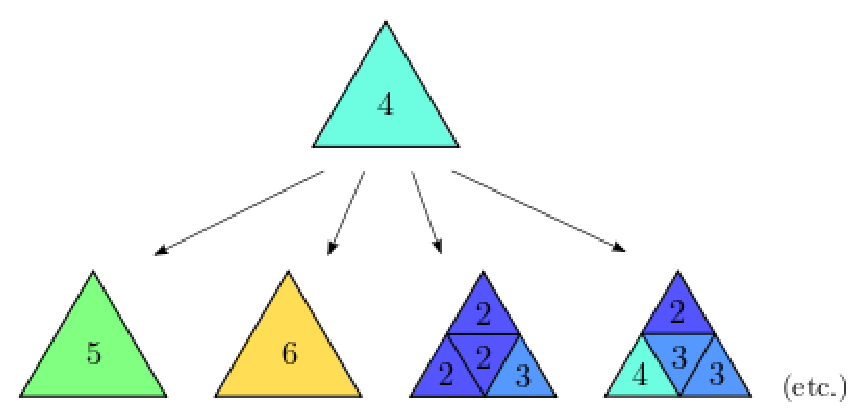
\includegraphics[width=0.5\columnwidth]{refinements}
  \caption{\label{fig:refinements} Many possible refinement candidates for a fourth-order
  element.}
  \end{centering}
%\vspace{-0.5cm}
\end{figure}

%\newpage
The number of possible element refinements is implementation dependent. 
In general it is very low in \emph{h}-adaptivity and \emph{p}-adaptivity, 
and much higher in \emph{hp}-adaptivity. Moreover, this number grows very 
fast when anisotropic refinements are enabled.

\subsection{The Hermes Library}

Hermes\footnote{http://hpfem.org/hermes} is a free and open-source C++ library 
that implements higher-order finite elements approximations and adaptive $hp$-FEM.
It supports 8 different adaptivity modes -- three isotropic and five anisotropic. 
The isotropic refinements are
\emph{h}-isotropic (H\_ISO), \emph{p}-isotropic (P\_ISO), \emph{hp}-isotropic (HP\_ISO).
Anisotropic refinement modes are
\emph{h}-anisotropic (H\_ANISO),
\emph{hp}-anisotropic-\emph{h} (HP\_ANISO\_H), \emph{p}-anisotropic (P\_ANISO),
\emph{hp}-anisotropic-p (HP\_ANISO\_P), and \emph{hp}-anisotropic (HP\_ANISO).
The eight adaptivity modes are summarized in Fig.~\ref{fig:candlist}. It must
be noted that in case of HP\_ANISO\_H, only element size is adapted anisotropically
whereas polynomial degree is adapted isotropically. The opposite holds true
for HP\_ANISO\_P.

\begin{figure}[!ht]
  \begin{centering}
  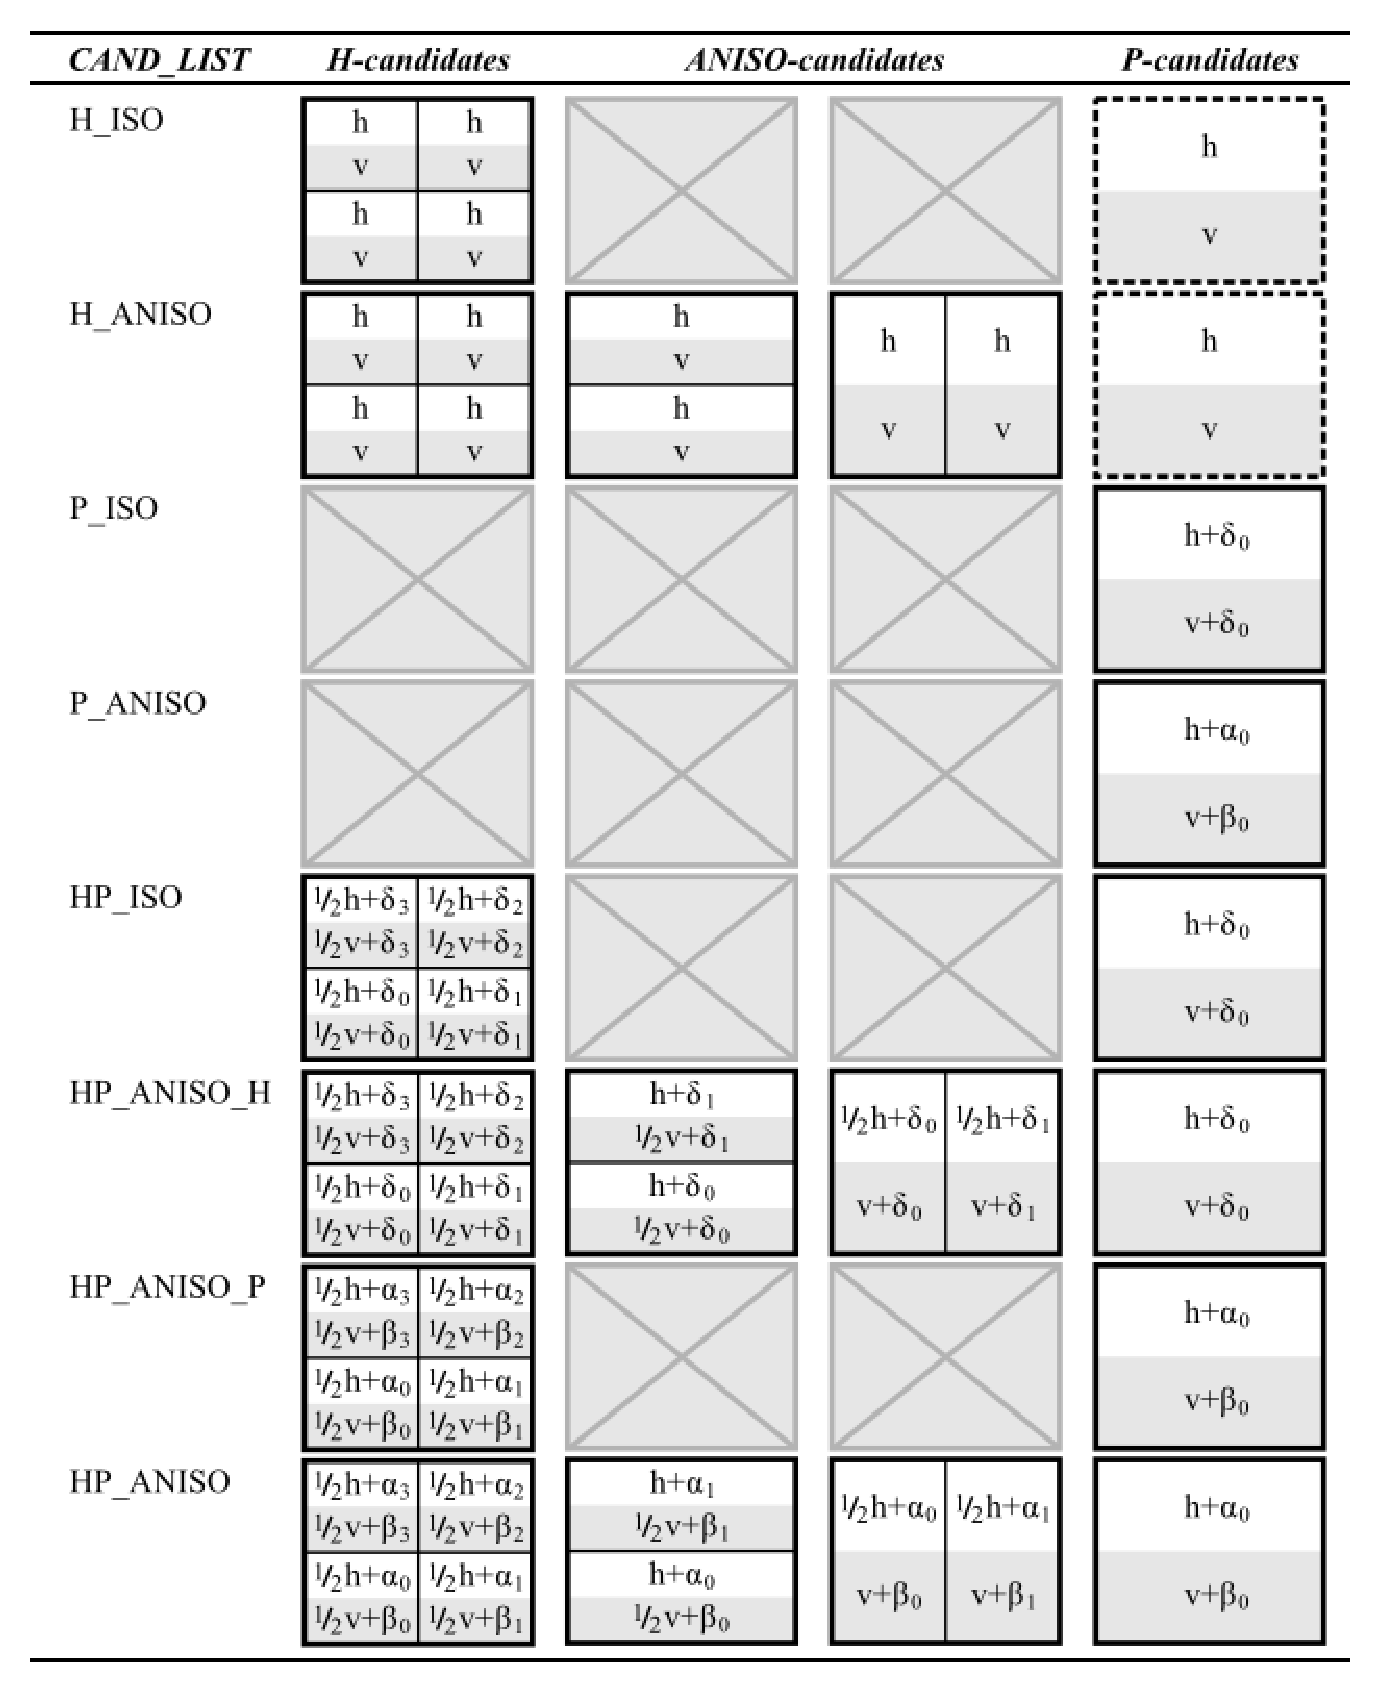
\includegraphics[width=0.8\columnwidth]{cand_list_quads}
  \caption{\label{fig:candlist} Refinement candidates for every
  refinement mode for quad type elements.}
  \end{centering}
\end{figure}
Note that triangular elements do not support anisotropic refinements.
Due to the large number of refinement options, classical error estimators 
that provide a constant error estimate per element, cannot be used to 
guide automatic \emph{hp}-adaptivity. 
For this, one needs to know the shape of the approximation error.
Hermes uses a pair of approximations with different orders of accuracy 
to obtain this information: coarse mesh solution and fine mesh solution~\cite{solin2010pde}. 
The initial coarse mesh is read from the mesh file, and the initial 
fine mesh is created through its global refinement both in \emph{h}
and \emph{p}. The fine mesh solution is the approximation of 
interest both during the adaptive process and at the end of computation. 
Global orthogonal projection of the fine mesh solution on the coarse mesh 
is used to extract the low-order part from the reference solution.
The adaptivity algorithm is guided by the difference between the 
reference solution and its low-order part.
% Pavel
% A short explanation, how Hermes further deals with this difference without
% going to much into details, might be interesting here...
Note that this approach to automatic adaptivity is PDE-independent
and thus naturally applicable to a large variety of multiphysics 
coupled problems.

\subsection{Multimesh $hp$-FEM}
In multiphysics PDE systems such as Poisson-Nernst-Planck it can 
happen that one physical field is very smooth where others are not,
as we illustrated in Fig.~\ref{fig:comsol-conc-volt}. 
If all the fields are approximated on the same mesh, then 
unnecessary refinements will be present in smooth areas
where they are not necessary. This can be very wasteful.

Hermes implements a novel adaptive multimesh $hp$-FEM~\cite{solin2010monolithic,
solin2010adaptive,dubcova2010space}
that makes it possible to approximate different fields on individual meshes,
without breaking the monolithic structure of the coupling mechanism.
For practical reasons, the meshes in the system are not allowed to be 
completely independent -- they have a common coarse mesh that we call {\em 
master mesh}. The master mesh is 
there for algorithmic purposes only and it may not even be used for 
discretization purposes. Every mesh in the system is obtained from 
the master mesh via an arbitrary sequence of elementary refinements. 
Assembling is done on a {\em union mesh}, a geometrical union of 
all meshes in the system (imagine printing all meshes on transparencies and 
positioning them on top of each other). 

The union mesh is not constructed physically in the computer 
memory -- it merely serves as a hint to correctly transform the 
integration points while integrating over sub-elements of elements 
in the existing meshes. 
As a result, the multimesh discretization of the PDE system is 
monolithic in the sense that no physics is lost --- all integrals 
in the discrete weak formulations are evaluated exactly up to 
the error in the numerical quadrature. The exact preservation of 
the coupling structure of multiphysics coupled problems makes 
the multimesh $hp$-FEM very different from various interpolation 
and projection based methods that suffer from errors made
while transferring data between different meshes in the system. 



\section{Results}

\begin{figure}
  \begin{centering}
  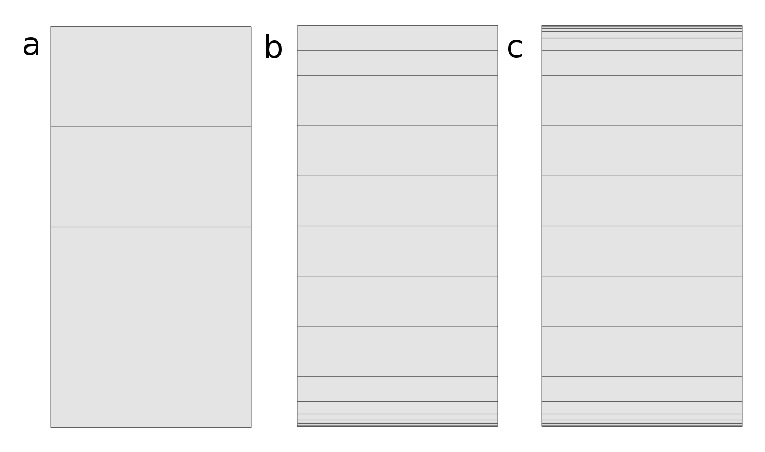
\includegraphics[width=.8\columnwidth]{mesh}
  \caption{\label{fig:mesh} Initial coarse mesh (a),
  	half refined mesh (b) and refined mesh (c). The coarse mesh
	and refined mesh were used in the initial calculations, the latter one
	in case of \emph{p}-adaptivity (including HP\_ANISO\_P). The half-refined mesh was
	used later to optimize the \emph{hp}-adaptive refinement solutions.}
  \end{centering}
\end{figure}
Calculation for all the refinement modes were performed
in both single-mesh and multi-mesh configurations. 
The following numerical results were recorded for each 
refinement mode: converged relative error, cumulative CPU
time, and the problem size in terms of number
of degrees of freedoms (NDOFs) at each time step. 
Two types of initial meshes were used --- in case of only \emph{p}-adaptivity,
more refined mesh was used (Fig.~\ref{fig:mesh}~(c)) to ensure
the error convergence.
When the element size refinement
was also enabled (all \emph{h}/\emph{hp} refinement modes), very coarse initial mesh
was used (see Fig.~\ref{fig:mesh}~(a)) to let the adaptivity
algorithm find the most optimal mesh. So coarse initial mesh might not be
suitable for all the practical applications, as will be demonstrated in the
end of this section, however, it provides a good insight into the
adaptivity performance of Hermes.
In both cases, the initial mesh was loaded at each time step of the
calculation.

\begin{figure}
  \begin{centering}
  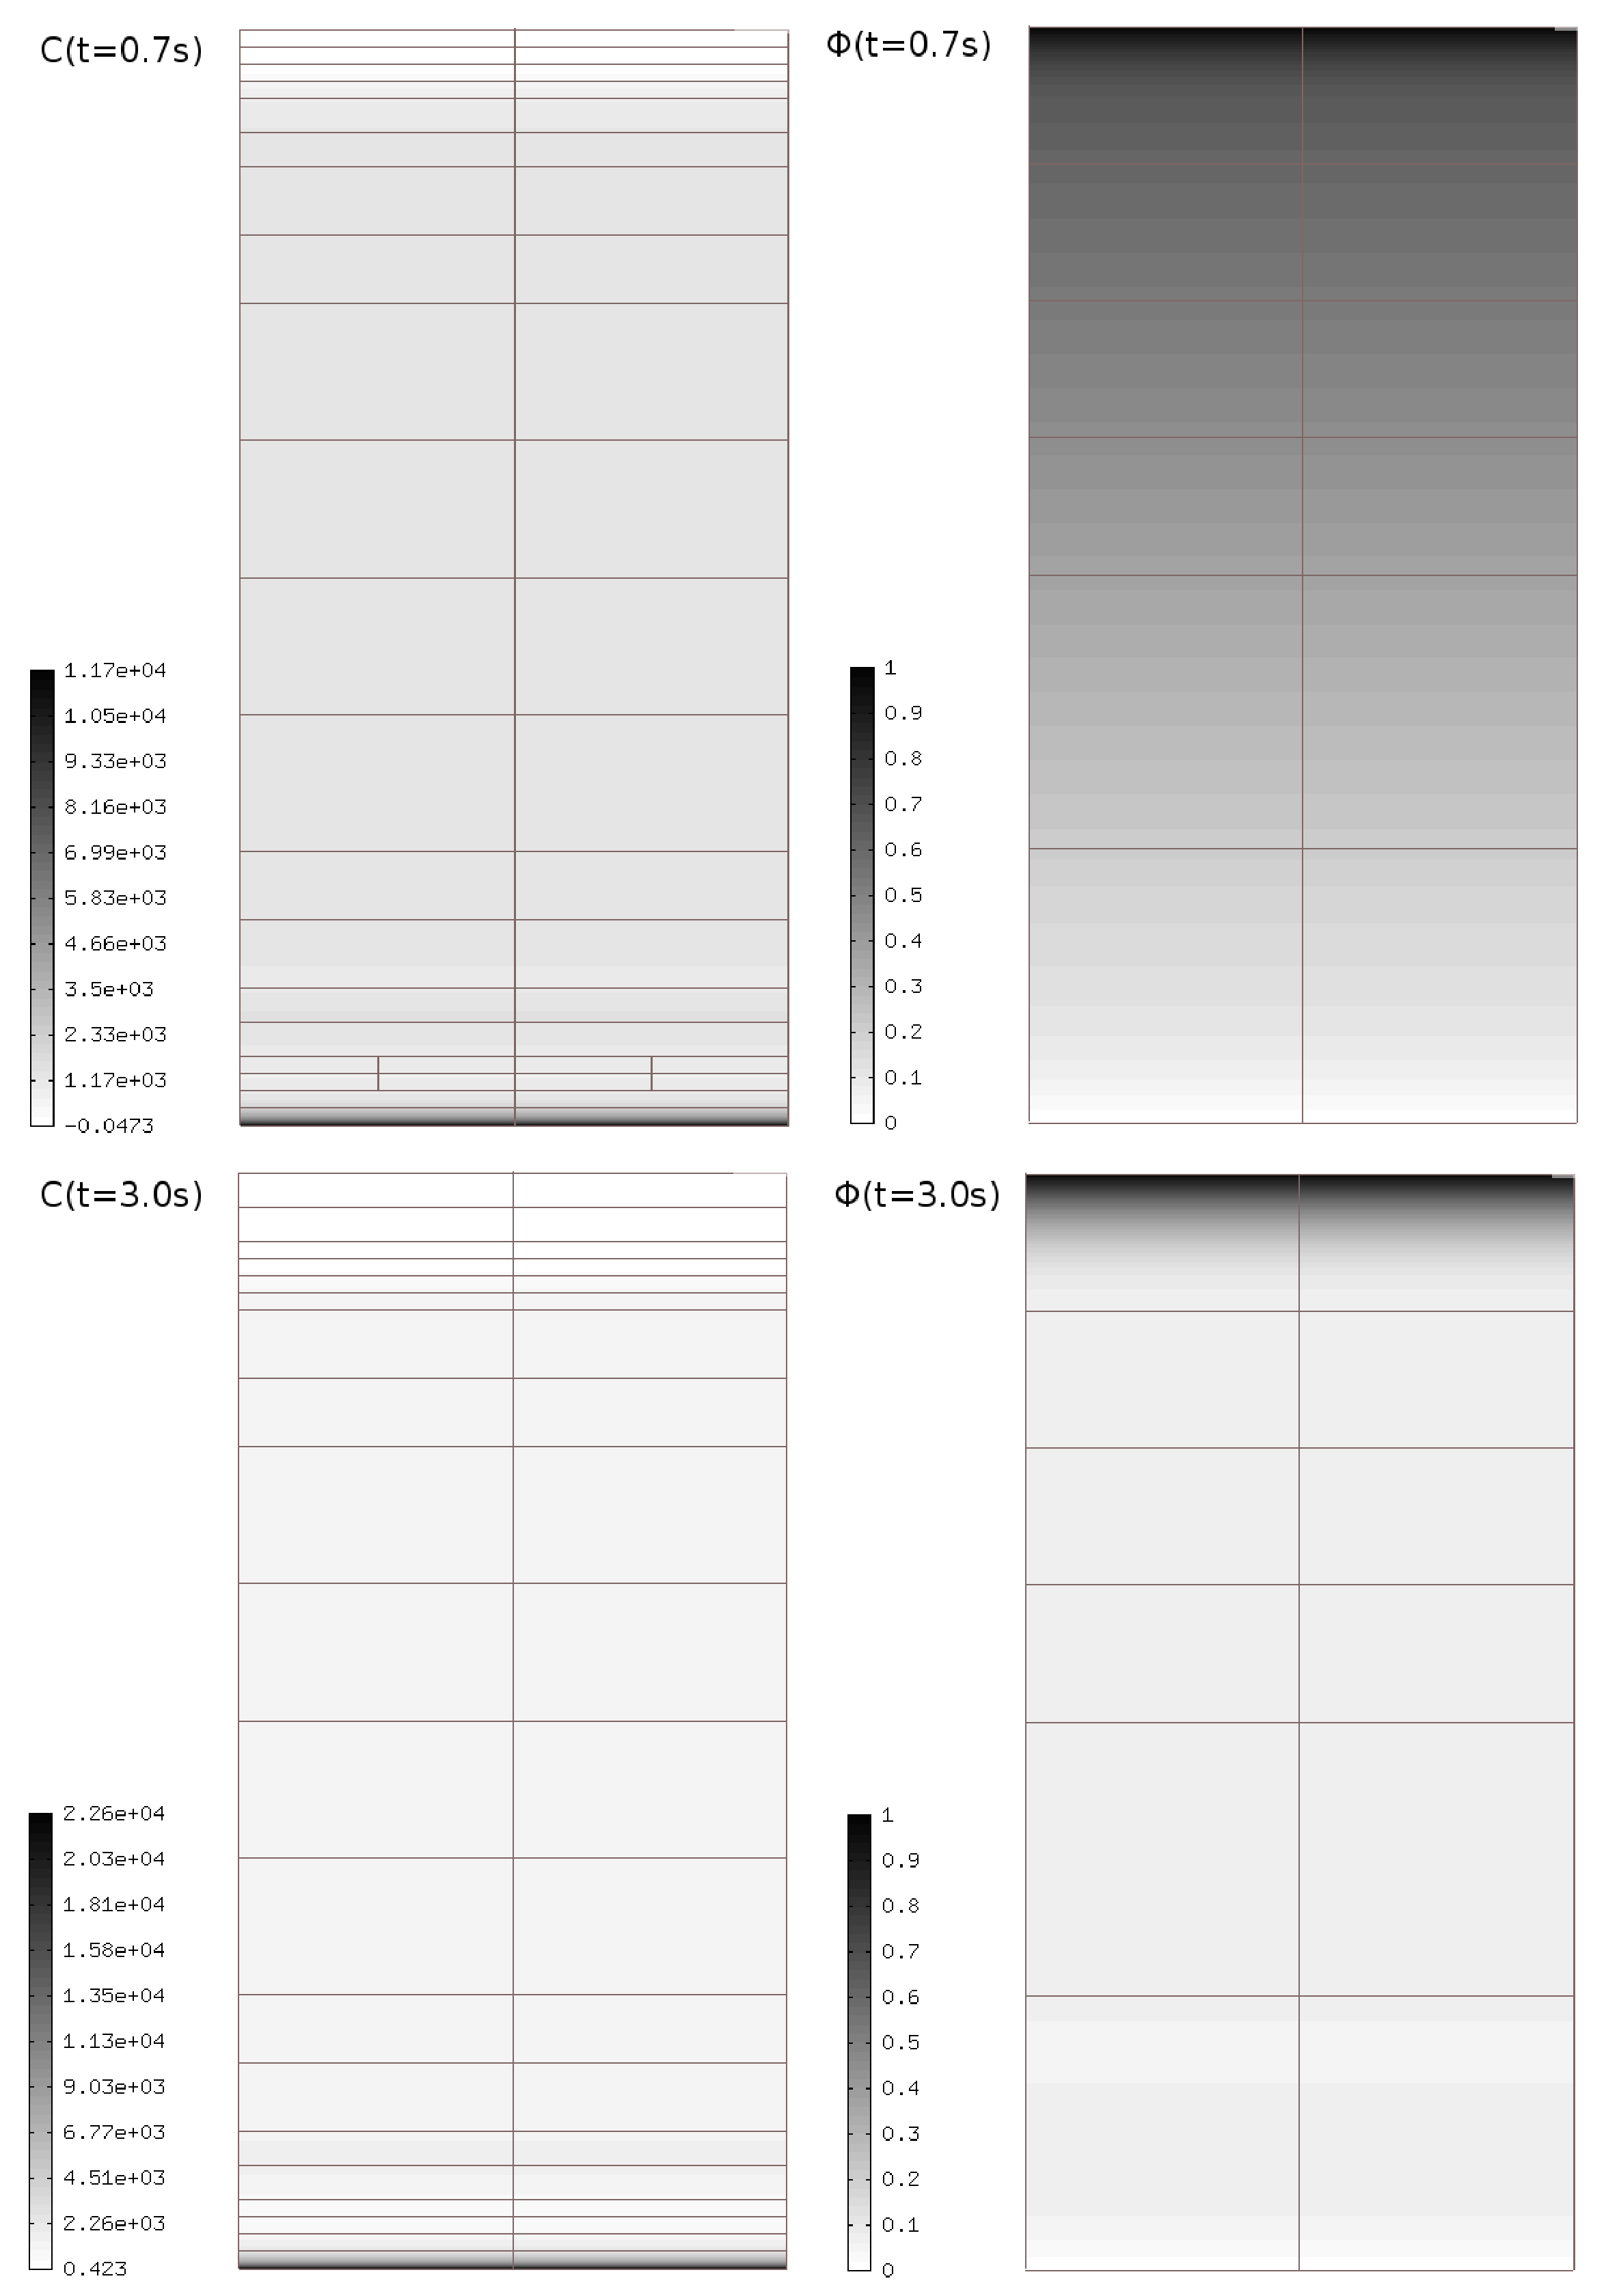
\includegraphics[width=.75\columnwidth]{cphi}
  \caption{\label{fig:cphi} Concentration $C$
  and voltage $\phi$ at two different time steps
  (HP\_ANISO adaptivity was used). This is a 2D solution shown
  as in 3D, where the height indicates the values of $C$ and $\phi$.}
  \end{centering}
\end{figure}
Example of the solution at $t=0.7\ s$ and $t=3.0\ s$ 
with refinement mode HP\_ANISO is shown
in Fig.~\ref{fig:cphi}. The time $t=0.7\ s$ was chosen because
by that time, some ionic migration has already taken place, i.e.
concentration gradient near the $\partial\Omega_1$ and
$\partial\Omega_3$ has formed. The automatic mesh refinements
at different time steps are clearly visible in the figure --- especially
near the top boundary, where the concentration gradient is
moving in time (as was also seen in Fig.~\ref{fig:comsol-conc-volt}).

The following subsections provide a detailed comparison of
the different refinement modes and try to estimate the most suitable
one for the given problem.

\subsection{Optimal refinement modes}

\begin{figure}
  \begin{centering}
  \includegraphics[width=\columnwidth]{singlemulti_dof}
  \caption{\label{fig:singlemultidof} NDOFs in case 
  of single-mesh and multi-mesh solutions with HP\_ISO
  and HP\_ANISO refinements. (Notice log Y scale)}
  \end{centering}
\end{figure}
\begin{figure}
  \begin{centering}
  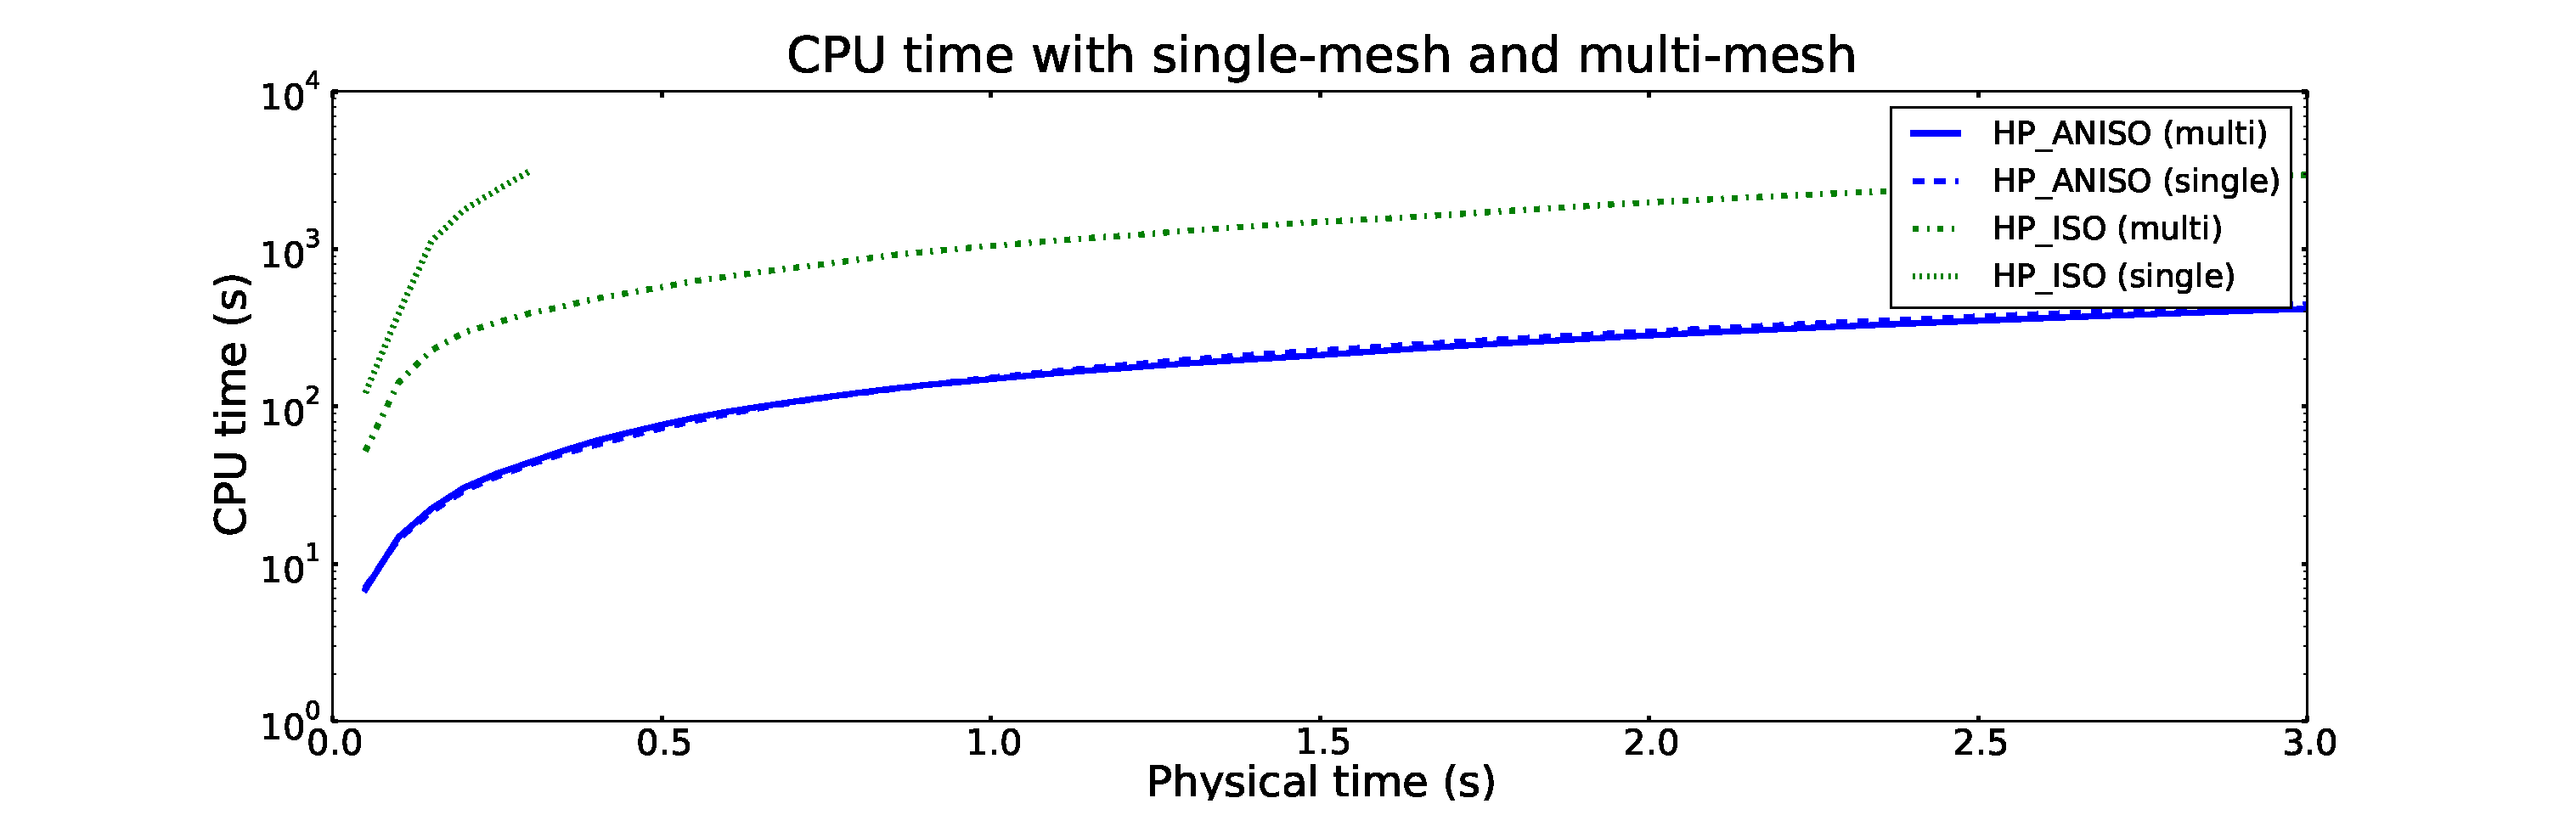
\includegraphics[width=\columnwidth]{singlemulti_cpu}
  \caption{\label{fig:singlemulticpu} CPU times in case
  of single-mesh and multi-mesh solutions with HP\_ISO
  and HP\_ANISO refinements. (Notice log Y scale)}
  \end{centering}
\end{figure}
\begin{figure}
  \begin{centering}
  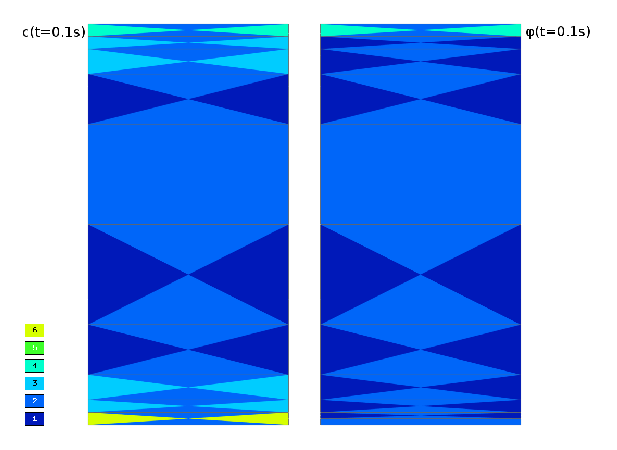
\includegraphics[width=.75\columnwidth]{poly}
  \caption{\label{fig:poly} Polynomial degree space
  for $C$ and $\phi$ at $t=0.7\ s$ The color indicates
  the maximum polynomial degree of the corresponding element.}
  \end{centering}
\end{figure}

Running the simulation with different refinement modes 
and meshes showed that the multi-mesh configuration generally results in
a smaller problem, faster calculation, and better or similar error convergence
compared to the single-mesh configuration.
This is well illustrated in Fig.~\ref{fig:singlemultidof} 
and Fig.~\ref{fig:singlemulticpu}.
The result can be understood from Fig.~\ref{fig:comsol-conc-volt} --- in the boundary
regions $\partial \Omega_1$ and $\partial\Omega_3$ the concentration gradient
is greater than voltage gradient, namely $\nabla C >> \nabla \phi$. Therefore
refining the mesh for both variables is not reasonable in terms of
number of degrees of freedom. For instance,
the solution space with corresponding mesh in case of
HP\_ANISO at $t=0.7\ s$ is shown in Fig.~\ref{fig:cphi}. The corresponding polynomial
degree space is shown in Fig.~\ref{fig:poly}. Notice that the adaptive algorithm
has increased the maximum polynomial degree for $C$ space to 7, however,
at the same time, the maximum polynomial degree for the $\phi$ space is one. Furthermore,
the mesh is significantly more refined for $C$.
For most cases using the multi-mesh results in similar or better CPU time, i.e.
multi-mesh takes less computational resources. Only excpetion was HP\_ANISO\_H 
refinement mode for which the single mesh configuration resulted slightly faster
calculation time. 
Based on the results, only multi-mesh configurations will be considered
in the following comparisons.

\begin{figure}
  \begin{centering}
  \includegraphics[width=\columnwidth]{isoaniso_dof}
  \caption{\label{fig:isoanisodof} NDOFs in case 
  of multi-mesh solutions with H\_ISO, H\_ANISO,
  HP\_ISO, HP\_ANISO, and single-mesh solution with HP\_ANISO\_H
  refinement modes. (Notice log Y scale)}
  \end{centering}
\end{figure}
\begin{figure}
  \begin{centering}
  \includegraphics[width=\columnwidth]{isoaniso_cpu}
  \caption{\label{fig:isoanisocpu} CPU times in case 
  of multi-mesh solutions with H\_ISO, H\_ANISO,
  HP\_ISO, HP\_ANISO, and single-mesh solution with HP\_ANISO\_H
  refinement modes. (notice log Y scale)}
  \end{centering}
\end{figure}
\begin{figure}
  \begin{centering}
  \includegraphics[width=\columnwidth]{isoanisop_dof}
  \caption{\label{fig:isoanisopdof} NDOFs in case 
  of multi-mesh solutions with P\_ISO, P\_ANISO, and
  HP\_ANISO\_P refinement modes.}
  \end{centering}
\end{figure}
\begin{figure}
  \begin{centering}
  \includegraphics[width=\columnwidth]{isoanisop_cpu}
  \caption{\label{fig:isoanisopcpu} CPU times in case 
  of multi-mesh solutions with P\_ISO, P\_ANISO, and
  HP\_ANISO\_P refinement modes.}
  \end{centering}
\end{figure}
To narrow down the list of refinement modes for the given problem, first the
isotropic and anisotropic adaptivities were compared. The \emph{p}-adaptivity
modes were compared separately as they used more refined mesh (Fig.~\ref{fig:mesh}~(c)).
Fig.~\ref{fig:isoanisodof} and Fig.~\ref{fig:isoanisocpu} show the comparison
of H\_ISO, H\_ANISO, HP\_ISO, HP\_ANISO, and HP\_ANISO\_H modes in terms of CPU time
and problem size.
Fig.~\ref{fig:isoanisopdof} and Fig.~\ref{fig:isoanisopcpu} show the similar
comparsion for the P\_ISO, P\_ANISO, and HP\_ANISO\_P modes.
It can be clearly seen that the anisotropic refinement modes result in a reasonable problem
size and the problems solve within a reasonable calculation time. It is interesting
to note that HP\_ANISO results in the smallest problem size. Also, in
\emph{p}-adaptivity group, HP\_ANISO\_P results in the smallest problem size
at each time step, whereas P\_ISO and P\_ANISO have a very largy problem size
during the first time steps of the solution.
Here the term ``reasonable problem size''
means that the number of degrees of freedom in time converges
to so that $N_{dof}<500$, and the term ``reasonable calculation time''
means that the calculation (step $\tau=0.01\ s$, physical
time $t_{end}=3.0\ s$) time $t$ on a givem system was $t<500\ s$.
Although these parameters are empirical, they serve as an upper limit, given
that the most refinement modes give significantly smaller results:
$t<<500\ s$ and $N_{dof} << 500$.

\subsection{Quantitative analysis of the refinement modes}

Based on the results in the previous subsection, H\_ANISO, HP\_ANISO,
and HP\_ANISO\_H from the \emph{hp/h}-adaptivity group and HP\_ANISO\_P
from \emph{p}-adaptivity group will be compared
in terms of problem size and cumulative CPU time. 
In all of the cases, the relative 
error at each time step remained below
the threshold which were set to $e_{th}=0.5\%$ between the coarse mesh
and fine mesh solutions, therefore the error-time plot will not be considered.

\begin{figure}
  \begin{centering}
  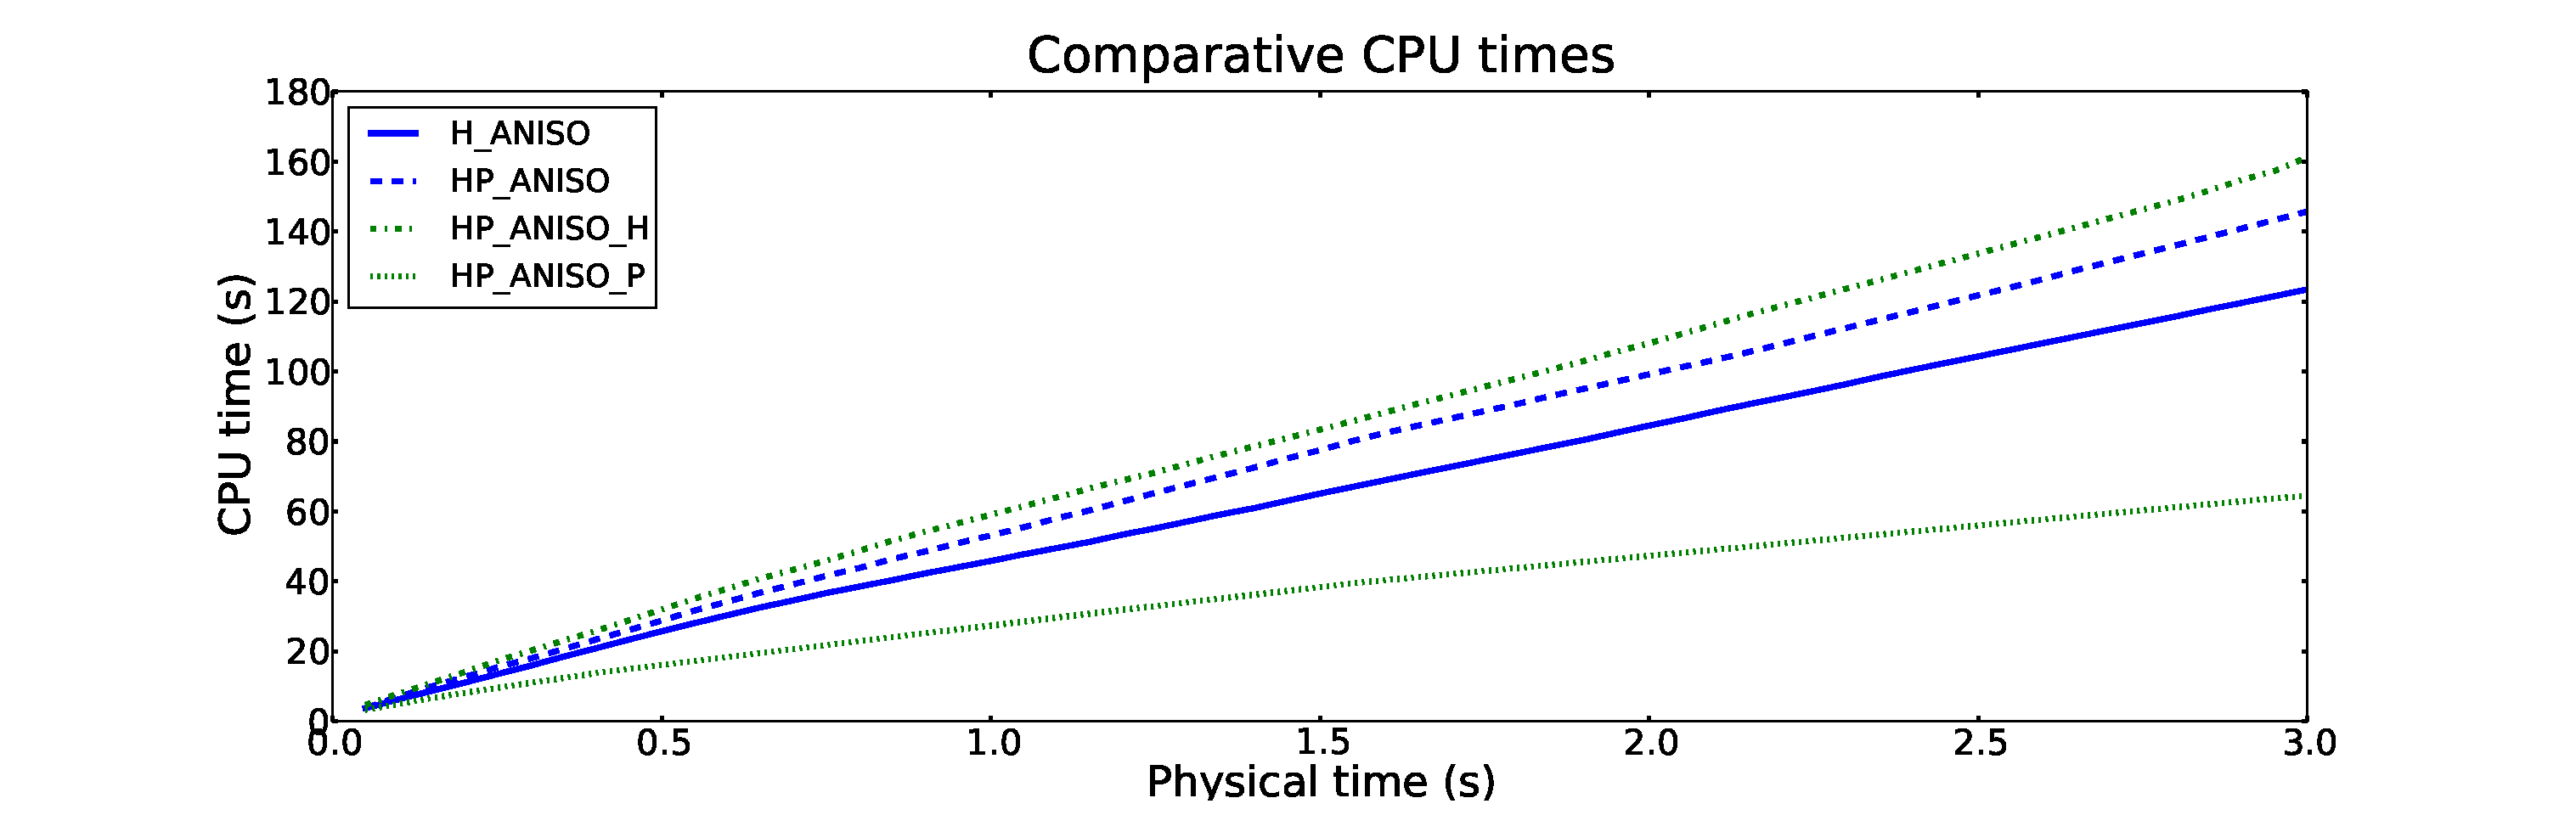
\includegraphics[width=\columnwidth]{cpu}
  \caption{\label{fig:cpu} Comparative CPU time for different refinement modes.}
  \end{centering}
\end{figure}

\begin{figure}
  \begin{centering}
  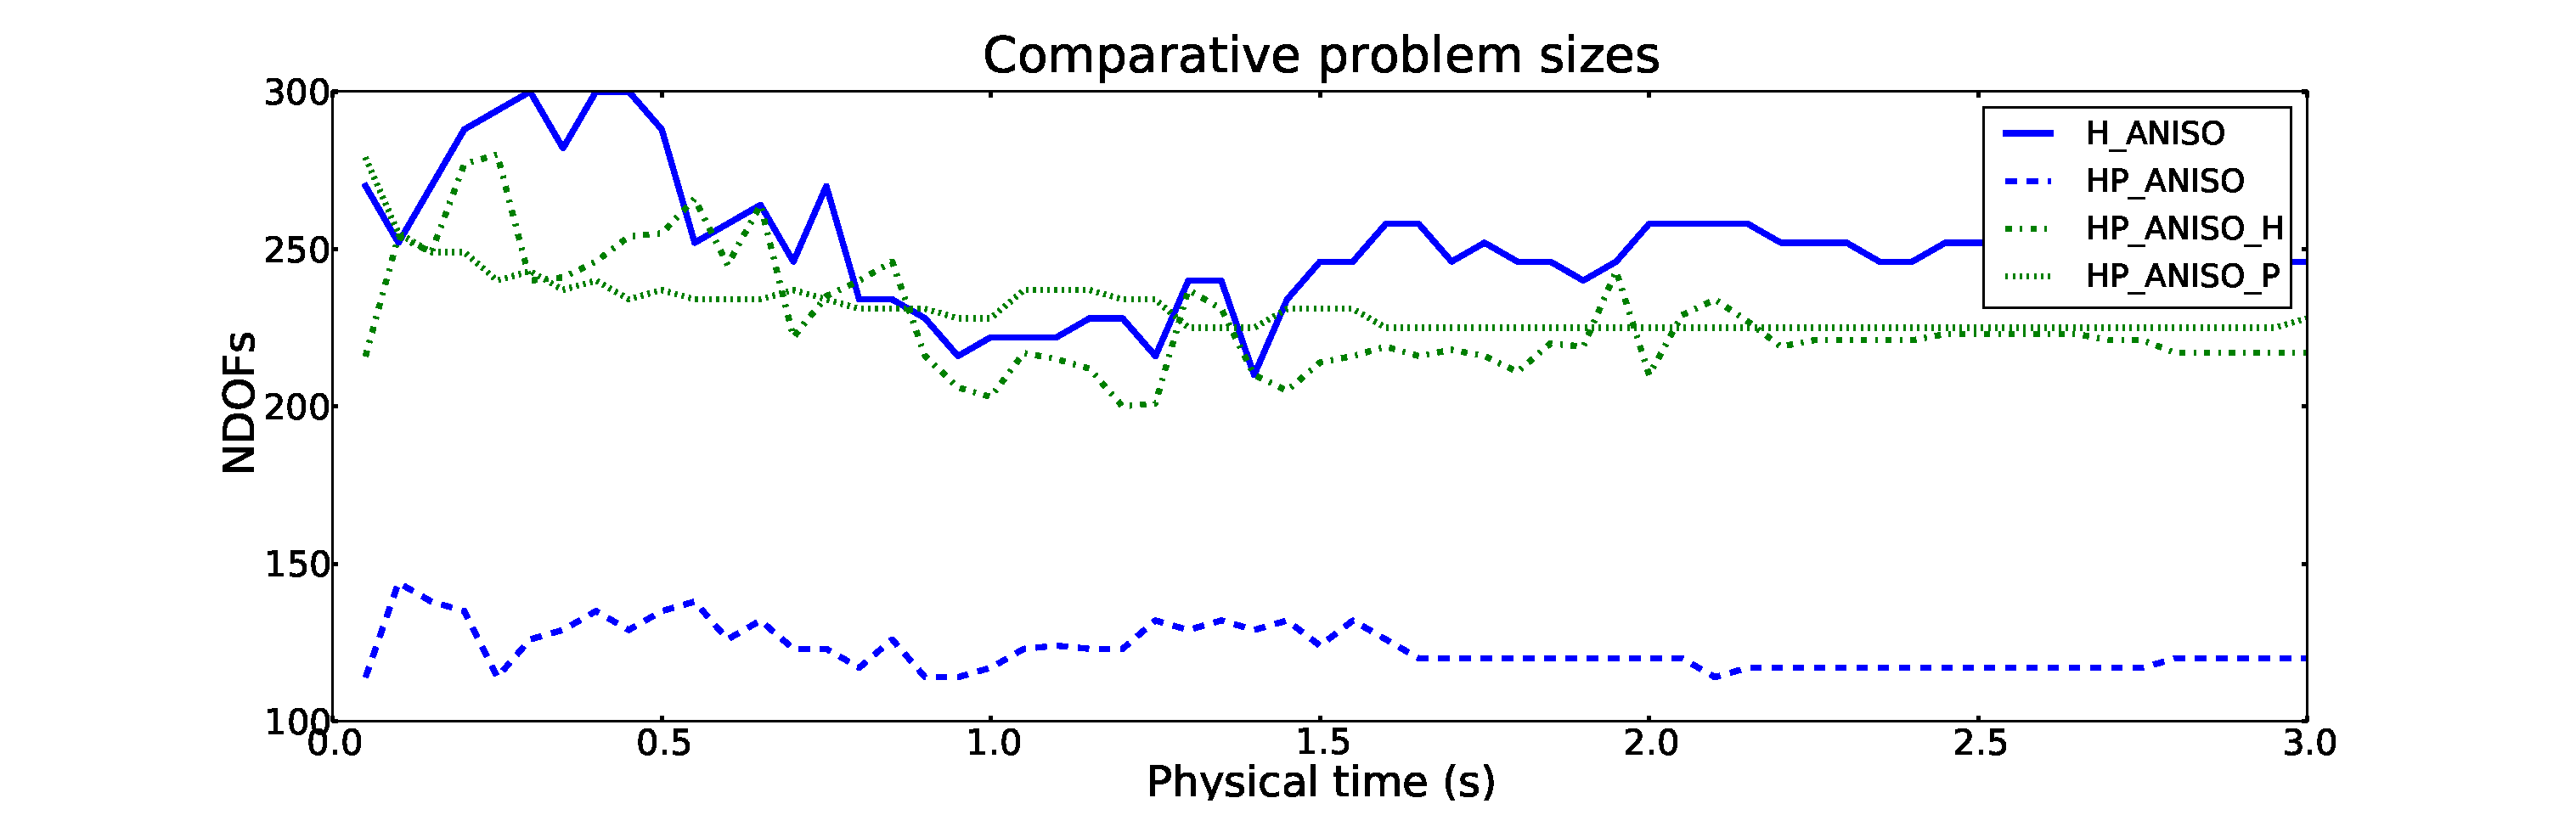
\includegraphics[width=\columnwidth]{dof}
  \caption{\label{fig:dof} Comparative NDOFs at each time step for 
  different refinement modes.}
  \end{centering}
\end{figure}

Fig.~\ref{fig:cpu} shows the cumulative CPU time for different refinement 
modes at each time step. All the calculations were done on the same computer.
Here we see that HP\_ANISO\_H and HP\_ANISO require the most
resources which can be understood from the fact that these 
refinement modes have the largest number of 
candidates (see Section.~\ref{sec:model}) from which the refinement method is chosen.
At the same time, HP\_ANISO\_P is the fastest among all the other refinement modes.
Fig.~\ref{fig:dof} shows the NDOFs at each time step.
It can be seen that the HP\_ANISO results in the 
smallest problem size --- $N_{dof} \approx 125$. 
All the other refinement modes result in a 
problem size of approximately ($N_{dof} \approx 250$). So we have
two notable refinement modes --- HP\_ANISO\_P because of the fast
solution, and HP\_ANISO because of the small problem size. In the following
subsection, optimization of those two modes will be considered.


\subsection{Optimizations of HP\_ANISO and HP\_ANISO\_P refinement modes}

\begin{figure}
  \begin{centering}
  \includegraphics[width=\columnwidth]{refined_cpu}
  \caption{\label{fig:refined-cpu} Cumulative CPU time for HP\_ANISO and HP\_ANISO\_P
  with different initial meshes.}
  \end{centering}
\end{figure}

\begin{figure}
  \begin{centering}
  \includegraphics[width=\columnwidth]{refined_dof}
  \caption{\label{fig:refined-dof} NDOFs at each time step for
  HP\_ANISO and HP\_ANISO\_P with different meshes.}
  \end{centering}
\end{figure}

So far we have seen that HP\_ANISO results in the smallest problem size, but requires
quite a lot CPU time compared to HP\_ANISO\_P that is the fastest.
When it comes to a large domain or 3D modeling the problem
size becomes the most important factor. Therefore, we consider HP\_ANISO the most
suitable refinement mode to the given problem. Thus some ways to optimize the time
factor will be considered. The desirable output would be HP\_ANISO problem size
close to HP\_ANISO\_P CPU time. One way to optimize the problem
is to choose somewhat more refined initial mesh. Other way one could think
to optimize the problem would be to change
the refinement frequency during the solving process. Recall that up to this point,
the initial mesh has been loaded in the beginning of each time step. True,
by employing the optimizations, we already must know something about the problem
and its solution beforehand. However, it could still be practial when solving a real problem
in a large domain.

The problem size and CPU time with HP\_ANISO
and HP\_ANISO\_P adaptivities on more refined initial mesh (see Fig.~\ref{fig:mesh}~(c))
compared to the coarse initial mesh (Fig.~\ref{fig:mesh}~(a)) and 
HP\_ANISO\_P solution is shown in Fig.~\ref{fig:refined-cpu} and Fig.~\ref{fig:refined-dof}.
By using initially more refined mesh, the problem solving time
can be reduced in case of HP\_ANISO, at the same time, the problem size increases.
In this situation, HP\_ANISO\_P and HP\_ANISO perform equally well.

\begin{figure}
  \begin{centering}
  \includegraphics[width=\columnwidth]{unreffreq_dof}
  \caption{\label{fig:unreffreq-dof} NDOFs at each time step for
  HP\_ANISO and HP\_ANISO\_P with mesh unrefinement at each time step and at over each
  	time step after first $0.5\ s$ physical solution time.}
  \end{centering}
\end{figure}
The next proposed optimization involved changing the unrefinement frequency.
It is known that the concentration gradient $\nabla C$ changes the most in the initial phase
of the calculation, therefore, the unrefinement after each time step was performed
until $t=0.5\ s$ (physical time). After that, the
unrefinement was performed in $\Delta t = 0.10\ s$ interval.
However, this optimization did not result in a stable solution, i.e. the problem size 
does not remain steady, but starts to oscillate depending on the unrefinement
frequency. This is shown in 
Fig.~\ref{fig:unreffreq-dof}. 

Therefore varying the unrefinement frequency will
not likely result in desired results in real applications for given system of equation.
At the same time, by varying a mesh size, optimal initial mesh could be found
for both HP\_ANISO and HP\_ANISO\_P refinement modes.
	 
\subsection{More general results}
\begin{figure}
  \begin{centering}
  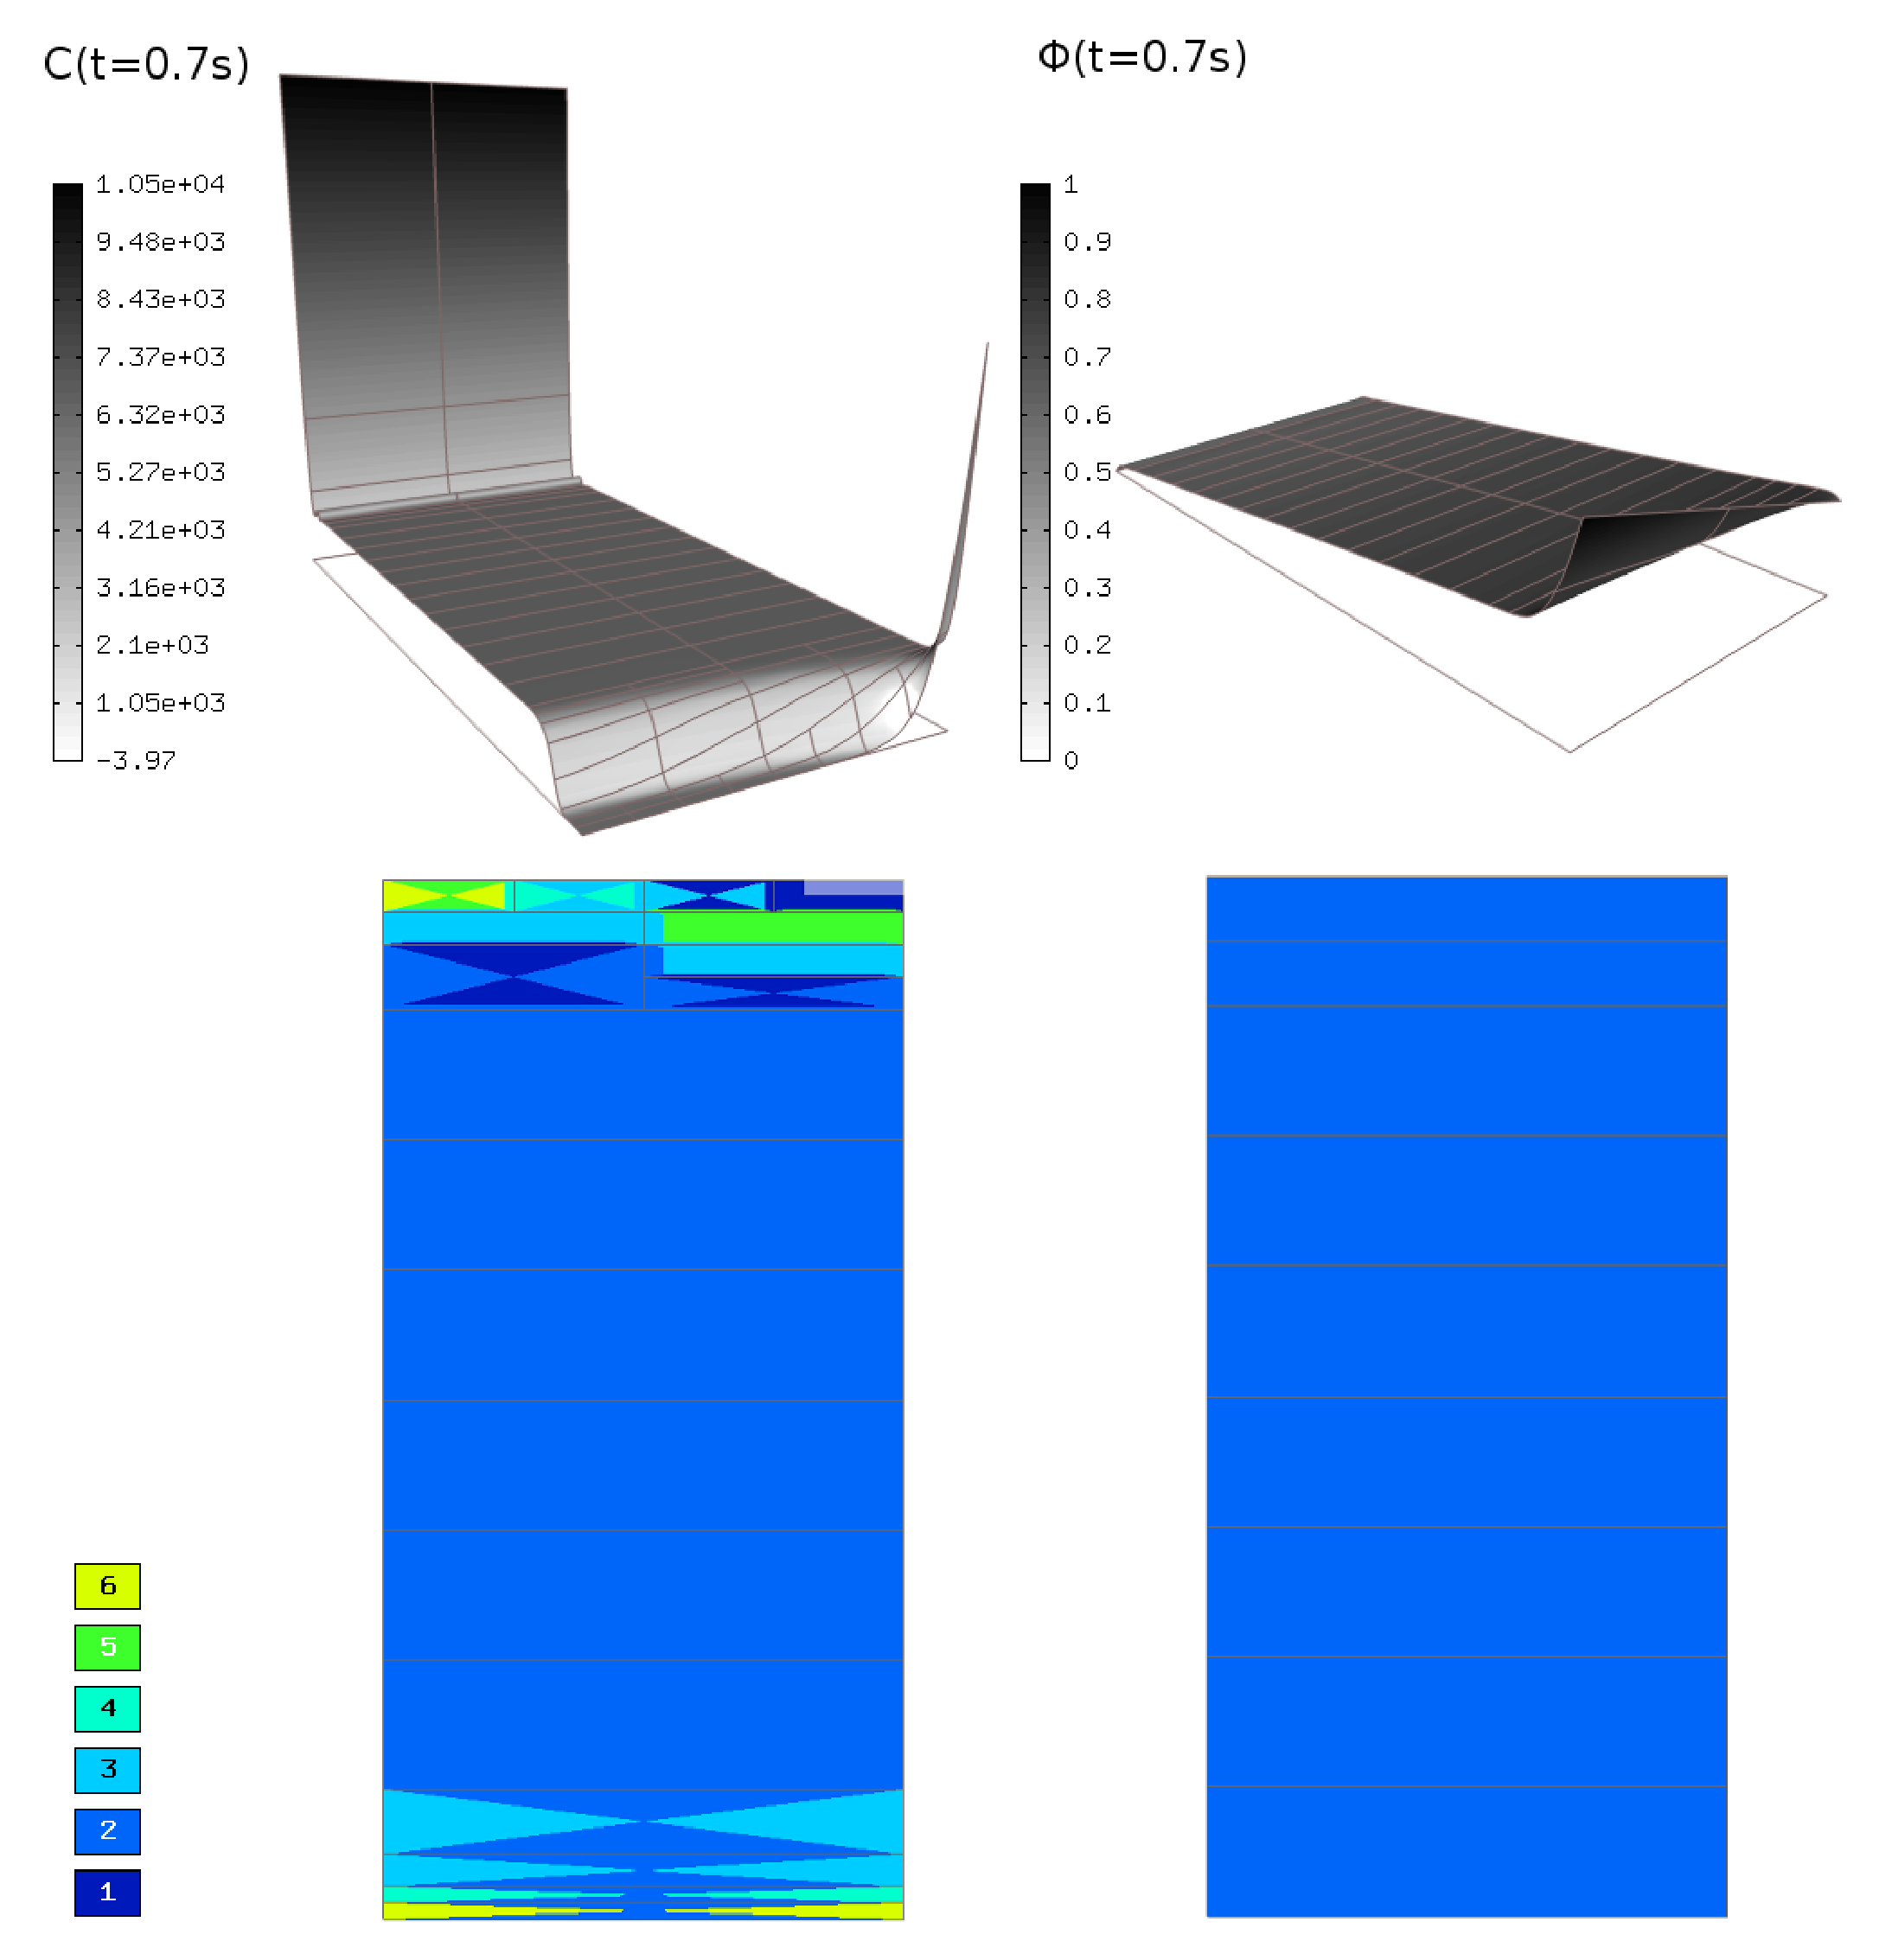
\includegraphics[width=.75\columnwidth]{cphiorders}
  \caption{\label{fig:cphi-orders} Solutions $C$ and $\phi$
  and corresponding polynomial degrees of the elements at
  $t=0.7\ s$. HP\_ANISO refinement mode was used. The height
  in the solution graphs indicates the value.}
  \end{centering}
\end{figure}

Based on the results, cation concentration and voltage was calculated
for different boundary conditions.
For instance, when voltage is applied as follows
\begin{equation}
  \phi_{\Omega_1}=0.5\frac{x}{width_{\Omega_1}}+0.5,
\end{equation}
the concentration gradient $\nabla C$ and the voltage gradient $\nabla \phi$ are no
longer effectively 1D.
The calculated $C$ and $\phi$ in $\Omega$ and corresponding meshes and polynomial
degrees of the elements are shown in Fig.~\ref{fig:cphi-orders}.
HP\_ANISO refinement mode was used. Notice that the solution
is different to the one in Fig.~\ref{fig:cphi} and the adapted mesh and the
polynomial degrees are also more complicated than in Fig.~\ref{fig:poly}.
It must be noted that in case of non uniform boundary conditions which
results in 2D problem, refined initial mesh was more efficient to use.

\emph{
PAVEL: Should I try to include the similar solution from comsol and do
some comparison here? I got this idea just before commiting the final
draft to you?}

\section{Conclusion and Outlook}\label{sec:conc}

In this work the system of Nernst-Planck-Poisson equations
was solved using \emph{hp}-finite element method with adaptive
multi-mesh configuration. The weak form, residuals and
the Jacobian matrix of the system were explicitly derived
and implemented in Hermes \emph{hp}-FEM time dependent
adaptive solver.
The solution for Nernst-Planck-Poisson
problem with two field variables $C$ and $\phi$ results in 
very different field gradients in the space and time.
When using a conventional low order
FEM, finding an optimal mesh for this
type of problem such that both the error of
the solution and problem size remain small throughout the
time dependent solving process is difficult. 

In the current work we showed that using the time dependent adaptivity, 
multi-mesh configuration, and anisotropic \emph{hp} refinements, the problem
size remains very small throughout the solving process while
maintaining a pre-set relative error of the solution.
Namely, Hermes refinement mode HP\_ANISO 
resulted in the smallest and fastest problem solution.
Furthermore, using the multi-mesh configuration for the physical fields
$c$ and $\varphi$ --- scaled variables for $C$ and $\phi$, respectively ---
was justified. The adaptivity algorithm
refined the meshes of $\varphi$  and $c$ and increased the
polynomial degrees of the corresponding spaces differently.
The mesh was significantly refined for $c$ and also the
maximum polynomial degree was varied in the range of
$2\ldots 9$ whereas for $\varphi$, the maximum polynomial degree
remained lower. So it is efficient to use multi-mesh in terms of
the number of degrees of freedom.

Conclusively, by using \emph{hp}-FEM with adaptive multi-mesh
configuration we can possibly reduce the problem size
of the Nernst-Planck-Poisson equation system significantly while
still maintaining prescribed precision of the solution. 
We believe, and this
is yet to be demonstrated, that this is especially
important when dealing with 3D problems in a large physical
domain with non-uniform boundary conditions.


\section*{Acknowledgments}
The second author was partially supported by the Grant Agency of the Academy of 
Sciences of the Czech Republic under Grant No. IAA100760702, and by the U.S.
Department of Energy Research Subcontract No. 00089911. 
The third author acknowledges the financial support of the U.S. Office of Naval Research 
under Award N000140910218. The fourth author acknowledges the financial support of
the Estonian Ministry of Education, grant \#SF0180008s08.

%\begin{thebibliography}{99}
%\bibitem{\ldots}..

%\end{thebibliography}
\newpage

\bibliographystyle{amsrn}    % Bibliography: Author-Date system
\bibliography{pugal-esco2010}      % pls. call your database here

\end{document}


